\documentclass[final,envcountsame]{llncs}


%\usepackage{graphicx} %Pouvoir inserer des images
\usepackage{epsfig}
\usepackage{amsmath} %Permet d'utiliser une jolie panoplie de symboles mathematiques
\usepackage{amssymb}
%\usepackage{amsthm}
\usepackage{stmaryrd}
\usepackage[ruled,vlined,linesnumbered]{algorithm2e}
\usepackage{amsfonts}


\newcommand{\centerness}{Decenter}

\def\OneBall#1{\mathbb{B}^{1}_{#1}}
\def\MaxOneBall#1{\mathbb{M}\OneBall{#1}}

\def\mydist1{D}
\def\mydd1{\Omega}
\def\mydecent{\mathcal{DC}}
\def\dist1{d}
\def\Dist1#1{\mydist1(#1)}
\def\DD1#1{\mydd1(#1)}
\def\decent#1{\mydecent(#1)}
\def\cplDist1#1{\mydist1^{cc}(#1)}
\def\cplDD1#1{\mydd1^{cc}(#1)}
\def\cpldecent#1{\mydecent^{cc}(#1)}


\def\mydef#1{{\em #1}}
\def\myem#1{{\em #1}}
\def\myvec#1{\vec{#1}}
\def\quotes#1{``#1''}

\def\birth#1#2{\mbox{\it{}Birth\/}_{#2}(#1)}
\def\death#1#2{\mbox{\it{}Death\/}_{#2}(#1)}
\def\lifespan#1#2{\mbox{\it{}Lifespan\/}_{#2}(#1)}


\def\V2C{\Psi}
\def\Nset{\mathbb{N}}
\def\Zset{\Z}
\def\Nset{\mathbb{N}}
\def\Rset{\mathbb{R}}
\def\Z{\mathbb{Z}}
\def\Zhalf{\frac{\mathbb{Z}}{2}}
\def\allfaces#1{\mathbb{F}^{#1}}
\def\subfaces#1#2{\allfaces{#1}_{#2}}
\def\subcomplex#1#2{#1 \preceq #2}
\def\complex#1#2{\subcomplex{#2}{\allfaces{#1}}}
\def\cell#1{\hat{#1}}
\def\cellstrict#1{\hat{#1}^*}
\def\closure#1{#1^-}
\def\princ#1{#1^+}
\def\mydim#1{\dim(#1)}
\def\type#1{\mbox{\it{}Dir\/}(#1)}
\def\orient#1{\mbox{\it{}Orient\/}(#1)}
\def\border#1{\mbox{\it{}Border\/}(#1)}
\def\suchthat{\;|\;}
\def\inter{\cap}
\def\union{\cup}
\def\dinterval#1#2{\{#1,\ldots,#2\}}
\newcommand{\Compl}[1]{\overline{#1}}
\def\finproof{\square}
\def\Zhalf{\frac{\mathbb{Z}}{2}}
\newcommand{\Card}[1]{|#1|}

\def\figpath{./images}

\def\figpath{images}
\def\myincludegraphics#1#2{\includegraphics[width=#1]{\figpath/#2}}



\begin{document}

\mainmatter

\title{A 3d curvilinear skeletonization algorithm with application to path tracing}
\author{John Chaussard\inst{1} \and Laurent No\"{e}l\inst{2} \and Venceslas Biri\inst{2} \and Michel Couprie\inst{2}\thanks{This work has been partially supported by the \quotes{ANR-2010-BLAN-0205 KIDICO} project}}
\institute{Universit\'{e} Paris 13, Sorbonne Paris Cit\'{e}, LAGA, CNRS(UMR 7539), \\ F-93430, Villetaneuse, France \\ \email{chaussard@math.univ-paris13.fr}
\and
Universit\'{e} Paris Est, LIGM, A3SI-ESIEE \\ 2, boulevard Blaise Pascal, 93162 Noisy le Grand CEDEX, France \\ \email{laurent.noel@esiee.fr, v.biri@esiee.fr, michel.couprie@esiee.fr}}


\maketitle


\begin{abstract}
We present a novel 3d curvilinear skeletonization algorithm which produces filtered skeletons without needing any user input, thanks to a new parallel algorithm based on the cubical complex framework. We then propose a new path tracing algorithm which uses such curvilinear skeleton in order to produce less noisy images in less time than the classical approach.
\end{abstract}



%%%%%%%%%%%%%%%%%%%%%%%%%%%%%%%%%%%%%%%%%%%%%%%%%%%%%%%%%%
%                                                        %
%                   INTRODUCTION                         %
%                                                        %
%%%%%%%%%%%%%%%%%%%%%%%%%%%%%%%%%%%%%%%%%%%%%%%%%%%%%%%%%%
\section{Introduction}
\label{sec::intro}

Path tracing algorithms are able to render photorealistic images from a scene description by simulating light propagation. The photorealistic aspect is achieved by simulating diffusion of light: elements of the scene which are illuminated by a light source can cast part of the light they receive. Consequently, parts of the scene which are not directly illuminated by any light source actually receive light, thus giving a realistic effect of light diffusion to the resulting image. 

A path tracing algorithm sends rays (of light) from the camera (the viewpoint of the scene), and let them bounce around the scene until they encounter a directly illuminated zone. When a ray hits a point of an object (like a wall), it gathers information on the object's material. The ray is then reemitted in a random direction. Once a ray reaches a light source, the information it gathered through its journey in the scene is averaged in order to decide of the color of the first impact point. This color is then allocated to one of the pixels of the image, and the process is repeated for each pixel of the output image. To avoid \quotes{unrealistic} results due to an unusual reemission direction of a ray, the algorithm actually sends, for each pixel of the image, many rays: the more rays, the longer the algorithm will take to produce an image, but the more realistic the result will look. A path tracing can be seen as a random walk process through the scene.

In order to avoid infinite bouncing of rays in the scene, a limit is set for the number of bounces a ray can do. If a ray does not reach any light source after a given number of bounces, it is eliminated from the scene. A lost ray is as a waste of computation time, and minimizing this loss would speed up the algorithm.

Our proposition is to reduce both the time taken by a path tracing algorithms and the noise in the output images by guiding rays towards the scene's light sources, thus reducing the number of rays \quotes{lost} during the computation. To do this, we perform some precomputation on the void space of the scene (the medium where the rays of light propagate) in order to have, later in the algorithm, a clue on towards which direction a ray should bounce in order to meet a light source. Such precomputation can take time and become more expensive than the original algorithm.

To keep the precomputation fast, we perform it only on a subset of points of the voids of the scene. The precomputation we want to perform relies on paths and visibility tests, therefore want this set of points to be representative of both the topology and the geometry of the original scene. For example, it should possess branches propagating in the elongated parts of the scene. A filtered curvilinear skeleton of (the voids of) the scene meets all the required properties for our subset of points: it is a thin subset of points of the scene, with the same topology and retaining the main geometrical information of the scene. Note that in this application, the filtering of the skeleton (elimination of spurious branches) need to be both efficient and completely automatic, for one cannot ask a user to set parameters for each scene. 

\begin{figure}[tb]
\begin{center}
\begin{tabular}{cc}
	\myincludegraphics{0.60\textwidth}{dgci_ray_corridor.png} &
	\myincludegraphics{0.40\textwidth}{dgci_compare_door.png}
\end{tabular}
\caption{Images $a$ and $b$ shows some rays of the path tracing guided by the material of the objects (image $a$) or our skeleton based method (image $b$). Images $c$ and $d$ point out the noise reduction between the classic path tracing (image $c$) and our method (image $d$)}
\end{center}
\end{figure}

The purpose of this paper is twofold: we first introduce a new curvilinear skeletonization algorithm (Sec.~\ref{sec::skeletonization}) in the cubical complex framework (Sec.~\ref{sec::binary_to_cubic}), producing filtered skeletons without needing any user input (Sec.~\ref{sec::aspect_no_param}). 
Then, we expose a new method, based on such skeletons, to enhance the results and the performance of a path tracing algorithm (see Sec.~\ref{sec::appli_pathtrace}).

\section{The cubical complex framework}
\label{sec::binary_to_cubic}

In the 3d voxel framework, objects are made of voxels. In the 3d cubical complex framework, objects are made of cubes, squares, lines and vertices. 
Let $\Z$ be the set of integers, we consider the family of sets $\mathbb{F}^1_0$ and $\mathbb{F}^1_1$, such that $\mathbb{F}^1_0 = \{\{a\} \suchthat a \in \Z\}$ and $\mathbb{F}^1_1 = \{ \{a, a+1\} \suchthat a \in \Z\}$. Any subset $f$ of $\Z^n$ such that $f$ is the cartesian product of $m$ elements of $\mathbb{F}^1_1$ and $(n-m)$ elements of $\mathbb{F}^1_0$ is called a face or an \myem{$m$-face} of $\Z^n$, $m$ is the dimension of $f$, we write $dim(f)=m$. A $0$-face is called a \myem{vertex}, a $1$-face is an \myem{edge}, a $2$-face is a \myem{square}, and a $3$-face is a \myem{cube}.

We denote by $\allfaces{n}$ the set composed of all faces in $\Z^n$. Given $m \in \dinterval{0}{n}$, we denote by $\subfaces{n}{m}$ the set composed of all $m$-faces in $\Z^n$.
Let $f \in \allfaces{n}$. We set $\cell{f} = \{g \in \allfaces{n}\vert g \subseteq f\}$, and $\cellstrict{f} = \cell{f} \setminus \{f\}$. Any element of $\cell{f}$ (resp. $\cellstrict{f}$) is \myem{a face of $f$} (resp. \myem{a proper face of $f$}.
The \myem{closure} of a set of faces $X$ is the set $\closure{X}=\union\{\cell{f} \vert f \in X\}$.

\begin{definition}
A finite set $X$ of faces in $\allfaces{n}$ is a \myem{complex} if $X=\closure{X}$, and we write $\complex{n}{X}$. 

Any subset $Y$ of $X$ which is also a complex is a \myem{subcomplex of $X$}, and we write $\subcomplex{Y}{X}$.
\end{definition}


%Informally, in 3d, a set of faces $X$ is a complex if each side (square) of a cube of $X$ also belong to $X$, each edge of a square of $X$ also belong to $X$, and each vertex of an edge of $X$ also belong to $X$. 

A face $f \in X$ is \myem{a facet of $X$} if $f$ is not a proper face of any face of $X$. The \myem{dimension of $X$} is $\mydim{X} = \max\{\mydim{f} \suchthat f \in X\}$. If $\mydim{X} = d$, then we say that $X$ is a $d$-complex.

Traditionally, a binary image is a finite subset of $\Zset^n$ (called voxel image when $n=3$). To transpose such image to the cubical complex framework, we associate to each element of $S\subseteq \Zset^n$ an n-face of $\allfaces{n}$. Let $x=(x_1,...,x_n) \in S$, we define the n-face $\V2C(x) = \{x_1, x_1 + 1\} \times \ldots \times \{x_n, x_n + 1\}$. We can extend the map $\V2C$ to sets: $\V2C(S)=\{\V2C(x) | x \in S\}$. Given a set $S \subset \Zset^n$, we associate to it the cubical complex $\closure{\V2C(S)}$.

The collapse operation is the basic operation for performing homotopic thinning of a complex, and consists of removing two distinct faces $(f,g)$ from a complex $X$ under the condition that they form a free pair:

\begin{definition}
Let $\complex{n}{X}$, and let $f,g$ be two faces of $X$. The face $g$ is \myem{free for $X$}, and the pair $(f,g)$ is \myem{a free pair for $X$} if $f$ is the only face of $X$ which strictly contains $g$. 
\end{definition}

It can be easily seen that if $(f,g)$ is a free pair for a complex $X$, then $f$ is a facet of $X$ and $\dim(g) = \dim(f)-1$.

\begin{definition}
Let $\complex{n}{X}$, and let $(f,g)$ be a free pair for $X$. The complex $X \setminus \{f,g\}$ is an \myem{elementary collapse of $X$}.

Let $\complex{n}{Y}$, the complex $X$ \myem{collapses onto} $Y$ if there exists a sequence of complexes $(X_0,...,X_\ell)$ of $\allfaces{n}$ such that $X=X_0$, $Y=X_\ell$ and for all $i \in \dinterval{1}{\ell}, X_{i}$ is an elementary collapse of $X_{i-1}$. We also say, in this case, that $Y$ \myem{is a collapse of} $X$.
\end{definition}

Recent works in the cubical complex framework brought new parallel thinning algorithms in the voxel framework (\cite{BertrandCouprie06}, \cite{Ber07}).

\section{A parallel directional thinning based on cubical complex}
\label{sec::skeletonization}

In the cubical complex framework, parallel removal of free pairs can be easily achieved when following simple rules that we give now. First, we need to define the \myem{direction} and the \myem{orientation} of a free face.
Let $(f,g)$ be a free pair for $\complex{n}{X}$ : we have $\mydim{g} = \mydim{f}-1$, and it can be seen that $g = f \inter f'$, where $f'$ is the translate of $f$ by one of the $2n$ vectors of $\Zset^n$ which have all their coordinates equal to 0 except one, which is either equal to +1 or -1. Let $v$ be this vector, and $c$ its non-null coordinate. We define $\type{f,g}$, called the \myem{direction} of the free pair $(f,g)$, as the index of $c$ in $v$. The \myem{orientation} of the free pair $(f,g)$ is defined as $\orient{f,g}=1$ if $c=1$, and $\orient{f,g}=0$ else.

%On Fig.~\ref{fig:parallel_collapse}, the free pair $(a,c)$ and the free pair $(d,e)$ have different directions; the free pairs $(a,b)$ and $(d,e)$ have the same direction, but different orientations.

Now, we give a property of collapse (previously proven in \cite{ChauCou2009}) which brings a necessary and sufficient condition for removing two free pairs of faces in parallel from a complex, while preserving topology.

\begin{proposition}
\label{prop:collpar2}
Let $\complex{n}{X}$, and let $(f,g)$ and $(k,\ell)$ be two distinct free pairs for $X$. The complex $X$ collapses onto $X \setminus \{f,g,k,\ell\}$ if and only if $f \neq k$. 
\end{proposition}

%\begin{proof}
%If $f=k$, then it is plain that $(k,\ell)$ is not a free pair for $Y=X \setminus \{f,g\}$ as $k=f \notin Y$. Also, $(f,g)$ is not free for $X \setminus \{k,\ell\}$. If $f\neq k$, then we have $g \neq \ell$, $\contstrict{g} \inter X = \{f\}$ ($g$ is free for $X$) and $\contstrict{\ell} \inter X = \{k\}$ ($\ell$ is free for $X$). Thus, we have $\contstrict{\ell} \inter Y = \{k\}$ as $\ell\neq g$ and $k\neq f$ and $(k,\ell)$ is a free pair for $Y$. $\finproof$
%\end{proof}

From Prop.~\ref{prop:collpar2}, the following corollary is immediate.

\begin{corollary}
\label{cor:parallel_removal}
Let $\complex{n}{X}$, and let $(f_1,g_1) \ldots (f_m,g_m)$ be $m$ distinct free pairs for $X$ such that, for all $a,b \in
\dinterval{1}{m}$ (with $a \neq b$), $f_a \neq f_b$. The complex $X$ collapses onto $X \setminus \{f_1,g_1 \ldots f_m,g_m\}$.
\end{corollary}

Considering two distinct free pairs $(f,g)$ and $(i,j)$ for $\complex{n}{X}$ such that $\type{f,g} = \type{i,j}$ and $\orient{f,g} = \orient{i,j}$, we have $f \neq i$.  From this observation and Cor.~\ref{cor:parallel_removal}, we deduce the following property.

\begin{corollary}
\label{cor:parallel_removal_v2}
Let $\complex{n}{X}$, and let $(f_1,g_1) \ldots (f_m,g_m)$ be $m$ distinct free pairs for $X$ having all the same direction and the same orientation. The complex $X$ collapses onto $X \setminus \{f_1,g_1 \ldots f_m,g_m\}$. 
\end{corollary}


Intuitively, we want our thinning algorithm to remove free faces of a complex \quotes{layer by layer} and to avoid having unequal thinning of the input complex. Therefore, we want each execution of the algorithm to remove free faces located on the border of the input complex. 
We define $\border{X}$ as the set all faces belonging to a free pair for $X$. We now introduce Alg.~\ref{algo::pardircollapse_v0}, a directional parallel thinning algorithm.

On a single execution of the main loop of Alg.~\ref{algo::pardircollapse_v0}, only faces located on the border of the complex are removed (l.~\ref{pc:07}). Thanks to corollary \ref{cor:parallel_removal_v2}, we can remove faces with same direction and orientation in parallel (l.~\ref{pc:08}), while guaranteeing topology preservation. Figure \ref{fig::example_algo} depicts the first steps of the algorithm.

\begin{algorithm}[tb]
\label{algo::pardircollapse_v0}
\SetKwFor{ForAll}{for all}{do}{end}
\caption[ParDirCollapse]{$ParDirCollapse(X,W,\ell)$}
\KwData{A cubical complex $\complex{n}{X}$, a subcomplex
  $\subcomplex{W}{X}$ which represents faces of $X$ which should not
  be removed, and $\ell \in \Nset$, the number of layers of free faces
  which should be removed from $X$} 
\KwResult{A cubical complex}
\lnl{pc:01}\While{there exists free faces in $X \setminus W$ and $\ell > 0$}{
\lnl{pc:02}  $L=\border{X}^-$\;
\lnl{pc:03}  \For{$t=0 \rightarrow n-1$}{
\lnl{pc:04}    \For{$s=0 \rightarrow 1$}{
\lnl{pc:05}      \For{$d=n \rightarrow 1$}{
\lnl{pc:06}        $E=\{(f,g)$ free for $X \suchthat g \notin W,$\\
                      $\;$~~~~~~~$\type{f,g}=t,$ $\orient{f,g}=s,$ $\mydim{f}=d\}$\;
\lnl{pc:07}        $G=\{(f,g) \in E \suchthat f \in L$ and $g \in L\}$\;
\lnl{pc:08}        $X=X \setminus G$\;
                 }
               }
             }
\lnl{pc:09}  $l = l-1$\;
	   }
\lnl{pc:10} \Return $X$\;
\end{algorithm}


\begin{figure}[tb]
\begin{center}
\begin{tabular}{ccccc}
	\myincludegraphics{0.19\textwidth}{invader.pdf} &
	\myincludegraphics{0.19\textwidth}{invader_step1_2.pdf} &
	\myincludegraphics{0.19\textwidth}{invader_step2_2.pdf} &
	\myincludegraphics{0.19\textwidth}{invader_step3.pdf} &
	\myincludegraphics{0.19\textwidth}{invader_step4.pdf} \\
\end{tabular}
\caption[Four first iterations of Alg.~\ref{algo::pardircollapse_v0}]{\label{fig::example_algo} \textbf{Four first iterations of Alg.~\ref{algo::pardircollapse_v0}} running on the left-most shape.}
\end{center}
\end{figure}



Different definitions of orientation and direction can be given, each corresponding to a different order of free faces removal in the complex and leading to different results.
Algorithm~\ref{algo::pardircollapse_v0} can be implemented to run in linear time complexity (proportionally to the number of faces in the complex). Indeed, checking if a face is free or not may be easily done in constant time and when a free pair $(f,g)$ is removed from the input complex, it is sufficient to scan the faces contained in $f$ in order to find new free faces.



\section{Aspect preservation during thinning}
\label{sec::aspect_no_param}
As previously said, our goal is to use the skeleton of the voids of a scene in order to guide light rays from the camera of the scene towards the light. Moreover, this skeleton needs to capture the main geometrical features of the original scene. For example, if the input is a corridor (the void of the corridor), then the skeleton should be a line following the main direction of the corridor.

Generally, two strategies are possible to achieve this goal: find, during the skeletonization process, points whose neighbourhood configuration seems interesting and keep them in the result \cite{CouCoeurZrour07} \cite{HR08} \cite{CCT09ext}), or choose, before skeletonization, interesting points of the object which should remain untouched, based on a function on these points and a filtering parameter \cite{BertrandCouprie06} \cite{Pal07}. 

Algorithm ~\ref{algo::pardircollapse_v0} does not necessarily preserve geometrical features of the input object in the resulting skeleton, which end up being a single vertex.

In the following, we introduce a new method in the cubical complex framework, requiring no user input, for obtaining a curvilinear skeleton yielding satisfactory geometrical properties. Our method is based on the two previously listed strategies: its finds, during thinning, elements whose neighbourhood configuration is interesting, and uses a function on these elements to decide to preserve them in the result.

\subsection{The lifespan of a face}
In the following, we define additional functions in the cubical complex, related to the thinning process (Alg.~\ref{algo::pardircollapse_v0}), which are essential for the filtering step of the skeletonization. The first one we present is the \myem{death date} of a face.

\begin{definition}
Let $f \in \complex{n}{X}$, the \myem{death date of $f$ in $X$}, denoted by $\death{f}{X}$, is the smallest integer $d$ such that $f \notin ParDirCollapse(X, \emptyset, d)$. 
\end{definition}

Intuitively, the death date of a face indicates how many layers of free faces should be removed from a complex $X$, using Alg.~\ref{algo::pardircollapse_v0}, before removing completely the face from $X$. We now define the \myem{birth date} of a face:

\begin{definition}
Let $f \in \complex{n}{X}$, the \myem{birth date of $f$ in $X$}, denoted by $\birth{f}{X}$, is the smallest integer $b$ such that either $f$ is a facet of $ParDirCollapse(X, \emptyset, b)$, or $f \notin ParDirCollapse(X, \emptyset, b)$.
\end{definition}

The birth date indicates how many layers of free faces must be removed from $X$ with Alg.\ref{algo::pardircollapse_v0} before transforming $f$ into a facet of $X$ (we consider that a face \quotes{lives} when it is a facet).
Finally, we define the \myem{lifespan} of a face :

\begin{definition}
Let $f \in \complex{n}{X}$, the lifespan of $f$ in $X$ is the integer 

\begin{math}
\lifespan{f}{X} = \left\{
\begin{array}{ll}
+\infty & \text{if $\death{f}{X}=+\infty$}\\
\death{f}{X} - \birth{f}{X} & \text{otherwise}
\end{array}
\right.
\end{math}
\end{definition}

These three values depend on the order of direction and orientation chosen for Alg.~\ref{algo::pardircollapse_v0}.

The lifespan of a face $f$ of $X$ indicates how many \quotes{rounds} this face \quotes{survives} as a facet in $X$, when removing free pairs with Alg.~\ref{algo::pardircollapse_v0}, and is a good indicator of how important a face can be in an object. Typically, the higher the lifespan is, and the more representative of an object's geometrical feature the face is. The lifespan, sometimes called \myem{saliency}, was used in \cite{Liu2009} (with the name \quotes{medial persistence}) in order to propose a thinning algorithm in cubical complexes based on two parameters.



\subsection{Distance map, opening function and decenterness map}
\label{subsec::distmap}
In addition to the lifespan of a face, the proposed homotopic thinning method uses information on distance between faces in order to decide if a face should be kept safe from deletion. We define hereafter various notions based on distances in the voxel framework.

Two points $x,y \in \Zset^n$ are \myem{$1$-neighbours} if the Euclidean distance between $x$ and $y$ is equal or inferior to $1$ (also called direct neighbours). A \myem{$1$-path from $x$ to $y$} is a sequence $\mathcal{C}=(z_0,...,z_k)$ of points of $\Zset^n$ such that $z_0=x$, $z_k=y$, and for all $j \in [1;k]$, $z_j$ and $z_{j-1}$ are $1$-neighbours. The length of $\mathcal{C}$ is $k$. 

We set $\dist1(x,y)$ as the length of a shortest $1$-path from $x$ to $y$; remark that $\dist1$ is indeed the $6$-distance in the 3d voxel framework. Let $S \subset \Zset^n$, we set $\Compl{S} = \Zset^n \setminus S$, and for all $x \in \Zset^n$, the map $\Dist1{S}: \Zset^n \rightarrow \Nset$ is such that $\Dist1{S}(x) = \displaystyle \min_{y \in \Compl{S}} \dist1(x,y)$. 

The \myem{maximal $1$-ball of $S$ centered on $x$} is the set $\MaxOneBall{S}(x)=\{y \in \Zset^n | \dist1(x,y) < \Dist1{S}(x)\}$.
We set, for all $x \in S$, the map $\DD1{S}: \Zset^n \rightarrow \Nset$ such that $\DD1{S}(x) = \displaystyle \max_{x \in \MaxOneBall{S}(y)} \Dist1{S}(y)$: this value indicates the radius of the largest maximal $1$-ball contained in $S$ and containing $x$. If $x \in \Compl{S}$, we set $\DD1{S}(x) = 0$. The map $\DD1{S}$ is known as the opening function of $S$ based on the $1$-distance (also called the granulometry function) \cite{Matheron67}: it allows to compute efficiently results of morphological openings by balls of various radius, and gives information on the local thickness of an object.

Given $S \subset \Zset^n$, the value of $\DD1{S}(x)$ of every $x \in S$ can be naively computed by performing successive morphological dilations of values of the map $\Dist1{S}$. A linear algorithm for computing the map $\DD1{S}$ (with regards to the size of the input image) was proposed in \cite{Chaussard_phd}, and will be explored further in details in a future paper.

Finally, we define the \myem{decenterness map}:

\begin{definition}
\label{def::decenterness_map}
Given $S \subset \Zset^n$, the \myem{decenterness map of $S$} is the map $\decent{S} = \DD1{S} - \Dist1{S}$.
\end{definition}

An exemple of these maps is shown on Fig.~\ref{fig::globalopening}.

In order to extend all these previous maps defined in $\Zset^n$ to the cubical complex framework, we use the map $\V2C^{-1}$, inverse of the bijective map $\V2C : \Zset^{n} \rightarrow \subfaces{n}{n}$ defined in Sec.~\ref{sec::binary_to_cubic}. It is used to project any $n$-face of $\allfaces{n}$ into $\Zset^n$. This map induces a map from $\mathcal{P}(\subfaces{n}{n})$ to $\mathcal{P}(\Zset^n)$, that we also denote by $\V2C^{-1}$.

Given $Y \subset \allfaces{n}$, we set $S = \V2C^{-1}(Y \inter \subfaces{n}{n})$. We define the map $\cplDist1{Y}: \allfaces{n} \rightarrow \Nset$ as follows: for all $f \in \allfaces{n}$,

\bigskip
\begin{math}
\cplDist1{Y}(f) = \left\{
\begin{array}{ll}
\Dist1{S}(\V2C^{-1}(f)) & \text{if $f$ is an $n$-face}\\
\displaystyle \max_{f \in (\cellstrict{g} \inter \subfaces{n}{n})} \cplDist1{Y}(g) & \text{otherwise}
\end{array}
\right.
\end{math}
\bigskip

Informally, if $f$ is a 3-face, then $\cplDist1{Y}(f)$ is the length of the shortest 1-path between the voxel \quotes{corresponding} to $f$ and the set of voxels corresponding to $Y$.
The same way, we define $\cplDD1{Y}$ and $\cpldecent{Y}$.

\begin{figure}[tb]
\begin{center}
\begin{tabular}{cccc}
	\myincludegraphics{0.22\textwidth}{fish.pdf} &
	\myincludegraphics{0.22\textwidth}{fishd.pdf} &
	\myincludegraphics{0.22\textwidth}{fishdd.pdf} &
	\myincludegraphics{0.22\textwidth}{fishcenter.pdf} \\
\end{tabular}
\caption[Example of opening and decenterness map]{\label{fig::globalopening} \textbf{Example of opening and decenterness map - } From left to right: a shape $S \subset \Zset^2$ (in gray), $\Dist1{S}$, $\DD1{S}$ and $\decent{S}$ (low values have dark colour).}
\end{center}
\end{figure}


\subsection{Parameter-free filtered thinning}
As previously said, we add edges to the set $W$ of Alg.~\ref{algo::pardircollapse_v0} in order to retain, in the resulting curvilinear skeleton, important edges from the original object. Given a cubical complex $X$, if an edge of $X$ has a high decenterness value for $X$, then it is probably located too close to the border of $X$ and does not represent an interesting geometrical feature to preserve.
On the other hand, if an edge has a high lifespan for $X$, then it means it was not removed quickly, after becoming a facet, by the thinning algorithm and might represent some precious geometrical information on the original object. An idea would be to keep, during thinning, all edges whose lifespan is superior to the decenterness value. Unfortunately, this strategy produces skeletons with many spurious branches in surfacic areas of the original object.

We can identify surfacic areas of a complex as zones where squares have a high lifespan. Therefore, in order to avoid spurious branches in surfacic areas, we need to make it harder for edges to be preserved in these zones. It can be achieved by deciding that an edge will be kept safe from deletion by the thinning algorithm if its lifespan is superior to the decenterness value plus the lifespan of squares \quotes{around} this edge. This leads us to proposing Alg.~\ref{algo::3d_curvskel}. 

\begin{algorithm}[tb]
\label{algo::3d_curvskel}
\caption[CurvilinearSkeleton]{$CurvilinearSkeleton(X)$}
\KwData{A cubical complex $\complex{3}{X}$}
\KwResult{A cubical complex $\complex{3}{Y}$}
\lnl{curvskel:01} $W=\{f \in X | \lifespan{f}{X} > \cpldecent{X}(f) + \birth{f}{X} - \cplDist1{X}(f)$ and $\mydim{f}=1\}$\;
\Return $ParDirCollapse(X,W,+\infty)$\;
\end{algorithm}

In order to understand what was realised on line \ref{curvskel:01} of Alg.~\ref{algo::3d_curvskel}, we might point out that the birth date of an edge corresponds to the highest death date of the squares containing this edge. Moreover, the map $\cplDist1{X}$ gives, for all 3-faces of $X$, their death date (as the thinning algorithm naturally follows this map to eliminate cubes from a 3-complex). Therefore, for an edge $f$ of $X$, $\cplDist1{X}(f)$ informs us on the highest death date of cubes containing $f$, also equal to the highest birth date of squares containing $f$. In conclusion, $\birth{f}{X} - \cplDist1{X}(f)$ is an approximation of the lifespan of the squares containing $f$.


\subsection{Results}

Algorithm \ref{algo::3d_curvskel} allows to obtain a filtered curvilinear skeleton from a three dimensional complex. The results presented in Fig.~\ref{fig::result_skel} show that the skeletons contain the main geometrical information from the input shapes, and no spurious branch.

\begin{figure}[tb]
\begin{center}
\begin{tabular}{cc|cc}
	\myincludegraphics{0.18\textwidth}{hand2.jpg} &
	\myincludegraphics{0.18\textwidth}{hand_curvskel.jpg} &
	\myincludegraphics{0.24\textwidth}{neptune.jpg} &
	\myincludegraphics{0.24\textwidth}{neptune_curvskel.jpg} \\
\end{tabular}
\caption[Results of algorithm \ref{algo::3d_curvskel}]{\label{fig::result_skel} \textbf{Results of algorithm \ref{algo::3d_curvskel}} for two shapes: a hand (left) and a statue (right). In each pair, the rightmost image represents the skeleton.}
\end{center}
\end{figure}




\section{Application to path tracing}
\label{sec::appli_pathtrace}

In this section, we explain how to use the curvilinear skeleton of the voids of the scene in order to enhance the path tracing algorithm. We start by defining some basic elements related to path tracing and we present our skeleton based path tracing algorithm.

%\subsection{Basic definitions of radiometry}
%
%Let $S$ be a set of surfaces of $\Rset^3$ that don't overlap and $S_L \subset S$ a set of surface lights. $S$ is called the scene.
%
%The basic radiometric quantity is the \myem{radiance} $L(x \rightarrow \Theta)$ that expresses the quantity of light energy produced by the surface point $x \in \Rset^3$ toward direction $\Theta \in \Omega_x$ per unit of time per unit area per unit solid angle (expressed in $W.m^{-2}.sr^{-1}$).
%This is the quantity that the eye actually "sees" and that must be computed for each pixel of the final image.
%
%% image radiance
%
%We can define another quantity related to radiance called \myem{incoming radiance} $L(x \leftarrow \Phi)$ that represents the radiance that reach $x$ from direction $\Phi$.
%
%In the void, incoming radiance can be written in terms of radiance as follow:
%
%\begin{equation*}
%L(x \leftarrow \Phi) = L(r(x, \Phi) \rightarrow -\Phi)
%\end{equation*}
%
%$r(x, \Phi)$ is the surface point seen by $x$ in the direction $\Phi$. It can be defined formally by:
%
%\begin{align*}
%r(x, \Phi) &= x + t_{min}\Phi \\
%t_{min} &= min \lbrace t \in (0, +\infty]~ |~ x + t\Phi \in S \rbrace
%\end{align*}
%
%If $t_{min} = \infty$ then $r(x, \Phi)$ is undefined and $L(x \leftarrow \Phi) = 0$. We call $r$ the \myem{raytrace} function. In practice it is implemented by throwing a ray in the scene and looking for the first intersection.
%
%A third quantity related to radiance is \myem{emitted radiance} $L_e(x \rightarrow \Theta)$. It is not null if $x$ is a point of a light source ($x \in S_L$). In practice the emitted radiance is given with the set $S_L$ as an input of the algorithm.
%
%The radiance is the solution of an equation called the Rendering Equation:
%
%\begin{align*}
%L(x \rightarrow \Theta) &= L_e(x \rightarrow \Theta) + \int_{\Phi \in \Omega_x} f_r(x, \Theta \leftrightarrow \Phi) L(x \leftarrow \Phi) cos(N_x, \Phi) d\omega_\Phi \\
%&= L_e(x \rightarrow \Theta) + L_r(x \rightarrow \Theta)
%\end{align*}
%
%This equation expresses an intuitive idea: the radiance produced by the point $x$ in the direction $\Theta$ is the sum of the emitted radiance and the reflected radiance.  The reflected radiance is computed by integrating the incoming radiance scaled by a factor $f_r(x, \Theta \leftrightarrow \Phi) cos(N_x, \Phi)$ over all the possible directions of the hemisphere around $x$. $N_x$ is the surface normal at point $x$.
%
%The $f_r$ function is called the \myem{bidirectional reflectance function} (BRDF) and express the exchange of radiance between the incoming direction $\Phi$ and the output direction $\Theta$. Intuitively it represents the material properties of the surface at point $x$. A mirror doesn't reflect light the same manners a wall do, the BRDF encodes that.
%
%It's actually the rendering equation that a path tracer try to resolve. Let $O$ be the origin of the camera and $I$ the image we want to compute (a rectangle embedded in $\Rset^3$). Then the path tracing algorithm compute an approximation of the radiances $L(O \leftarrow \vec{OP})$, $\forall P \in I$.

\subsection{The path tracing}

Let $O$ be the origin of the camera in the scene. For each pixel $P$ of the final image, let $x$ be the nearest intersection point of the ray $(O, \overrightarrow{OP} = -\Theta)$ with an element of the scene. To obtain the luminosity, we must solve the rendering equation \cite{Ka86} which is a recursive integral equation. The integrand of the equation contains the radiance function that we must compute:

\begin{align*}
L(x \rightarrow \Theta) &= L_e(x \rightarrow \Theta) + \int_{\Phi \in \Omega_x} f_s(x, \Theta \leftrightarrow \Phi) L(r(x, \Phi) \rightarrow -\Phi) d\omega_\Phi
\end{align*}

$L$ is the radiance (a radiometric quantity that represents luminosity) from point $x$ toward direction $\Theta$. $L_e$ is the emitted radiance (non null only on light sources). The point $r(x, \Phi)$ is the nearest visible point from $x$ in the direction $\Phi$ of the hemisphere $\Omega_x$. The $f_s$ function expresses how much luminosity is exchanged, on point $x$, between an incoming ray $\Phi$ and the outgoing ray $\Theta$. It represents the material properties of the surface at point $x$.

This integrand expresses an intuitive idea: the reflected radiance from $x$ towards the camera is the result of computing all incoming luminosity on $x$ scaled by a factor which depends on the material on $x$ and the angle of the ray going from the camera to $x$. The most common method used to estimate the integral, denoted by $L_r(x \rightarrow \Theta)$, is the Monte-Carlo integration which provides the following:

\begin{equation*}
\langle L_r(x \rightarrow \Theta) \rangle = \frac{f_s(x, \Theta \leftrightarrow \Phi) L(r(x, \Phi) \rightarrow -\Phi)}{p(\Phi)}
\end{equation*}

where $p$ is a probability density function (pdf) that is used to sample $\Phi$. This estimator is unbiased, meaning that the expected value $E[\langle L_r(x \rightarrow \Theta) \rangle]$ is equal to $L_r(x \rightarrow \Theta)$. The variance of the estimator expresses its quality and depends on the choosen pdf $p$. The best choice is a pdf that matches the shape of the function to integrate (ie. give high density to samples that have high values for the function and low density to samples that have low values).
The strategy of choosing an adapted pdf is called \myem{importance sampling} and is used in global illumination to improve the convergence speed of the algorithms.

The algorithm computes $L$ as follow: first, it chooses one random direction $\Phi$ based on the pdf $p$. Then, it applies the estimator by calling $L$ recursively to compute $L_r$ (shoots a new ray in the direction $\Phi$, computes the new hit point with the scene, and compute the new radiance at this point). Finally, it returns the sum of the emitted radiance $L_e$ and the result for $L_r$. The recursion stops when a maximal number of bounces has been reached.

This computation is done multiple times for each pixel (at different positions over the pixel). We average the results and get an estimation of the mean radiance passing through the pixel and heading towards the camera.
A bad pdf would lead in picking directions that don't reach the light before the end of the recursion, and produce results with a lot of noise in the final image. In the next part, we explain how to produce a pdf based on the curvilinear skeleton.



\subsection{Skeleton based importance sampling}

As stated in the introduction, a curvilinear skeleton of the void (with some preprocessing achieved on it) gives us information on which directions the light comes from. Given these directions, we can build a efficient pdf $p_{skel}$ and guide our rays by sampling the hemispheres with $p_{skel}$.

The integrand of $L_r$ is:

\begin{equation*}
f_s(x, \Theta \leftrightarrow \Phi) L(r(x, \Phi) \rightarrow -\Phi).
\end{equation*}

The most common strategy used to sample $\Omega_x$ is to use the function $f_s$ because it is an input of the algorithm.
The term $L$, which represents the distribution of light in the scene, is unknown. Our method gives a way to sample according to $L$.


\subsubsection{Construction of the importance points}

The skeleton of the voids of the scene is computed using Alg.~\ref{algo::3d_curvskel} (as shown on Fig.~\ref{fig::example_imp} on the right) and is converted to a graph (the nodes are the 0-faces and the edges are the 1-faces). We then compute a set of \myem{importance points}, which will be used to sample $\Omega_x$ in the path tracing algorithm. To each node $n$ of the skeleton, one importance point $imp_n$ is computed. Intuitively, the importance point associated to $n$ is the direction to follow in order to find a light source.

%La, pas clair !!!
Let $L$ be a light source of the scene and $n_L$ the nearest node of the skeleton that is visible by $L$. For each node, we compute the shortest path to $n_L$ along the skeleton. To do so, we use the Dijkstra algorithm and weight the edges of the skeleton depending on a visibility criteria: the weight of an edge $e$ is $1$ if $e$ is visible from $n_L$ and $10$ else. It results that the paths that are illuminated by a light will be shorter than paths located in dark areas.

Let $n$ be a node of the skeleton and $V_n$ the set of visible nodes from $n$ along the shortest path toward $n_L$. The importance point $imp_n$ associated to $n$ is the barycenter of $V_n$. An example is shown on Fig.~\ref{fig::example_imp} on the left.


\begin{figure}[tb]
\begin{center}
\begin{tabular}{l|r}
	\myincludegraphics{0.3\textwidth}{graph_heuristic.pdf} ~~~~~~&
	~~~~~~ \myincludegraphics{0.6\textwidth}{skel.jpg} \\
\end{tabular}
\caption[Example of importance point construction]{\label{fig::example_imp} \textbf{On the left}, we illustrate the importance point $imp_n$ associated to a node $n$. The dotted black line shows the closest node to $n$ not included in $V_n$. \textbf{On the right}, an example of the curvilinear skeleton (in red) obtained in the Sponza scene.}
\end{center}
\end{figure}


\subsubsection{Sampling according to $L$}

Given a point $x$ on the scene and a direction $\Theta$, we want to compute $L(x \rightarrow \Theta)$ and then sample the hemisphere $\Omega_x$. We search for the nearest skeleton node $n$ to $x$ and its importance point $imp_n$. We sample the hemisphere with a power-cosine pdf centered on $\overrightarrow{x\,imp_n}$:
\begin{equation*}
p_{skel}(\Phi) = \frac{s + 1}{2\pi} cos^s \alpha
\end{equation*}
with $\alpha$ the angle between $\overrightarrow{x\,imp_n}$ and $\Phi$, $s$ being a parameter called skeleton strength. The higher $s$ is, the closer to $\overrightarrow{x\,imp_n}$ we sample.


\subsection{Results and discussion}
Some results are presented on Fig.~\ref{fig:results} and Fig.~\ref{fig::intro_image} where we can see that our method produce less noisy images compared to the regular path tracing. We present, in table~\ref{tab:timing}, the time taken by each method to produce an image of same quality (the quality is measured by the mean square error (MSE) with a reference image) in different scenes.

\begin{figure}[tbhp]
\begin{center}
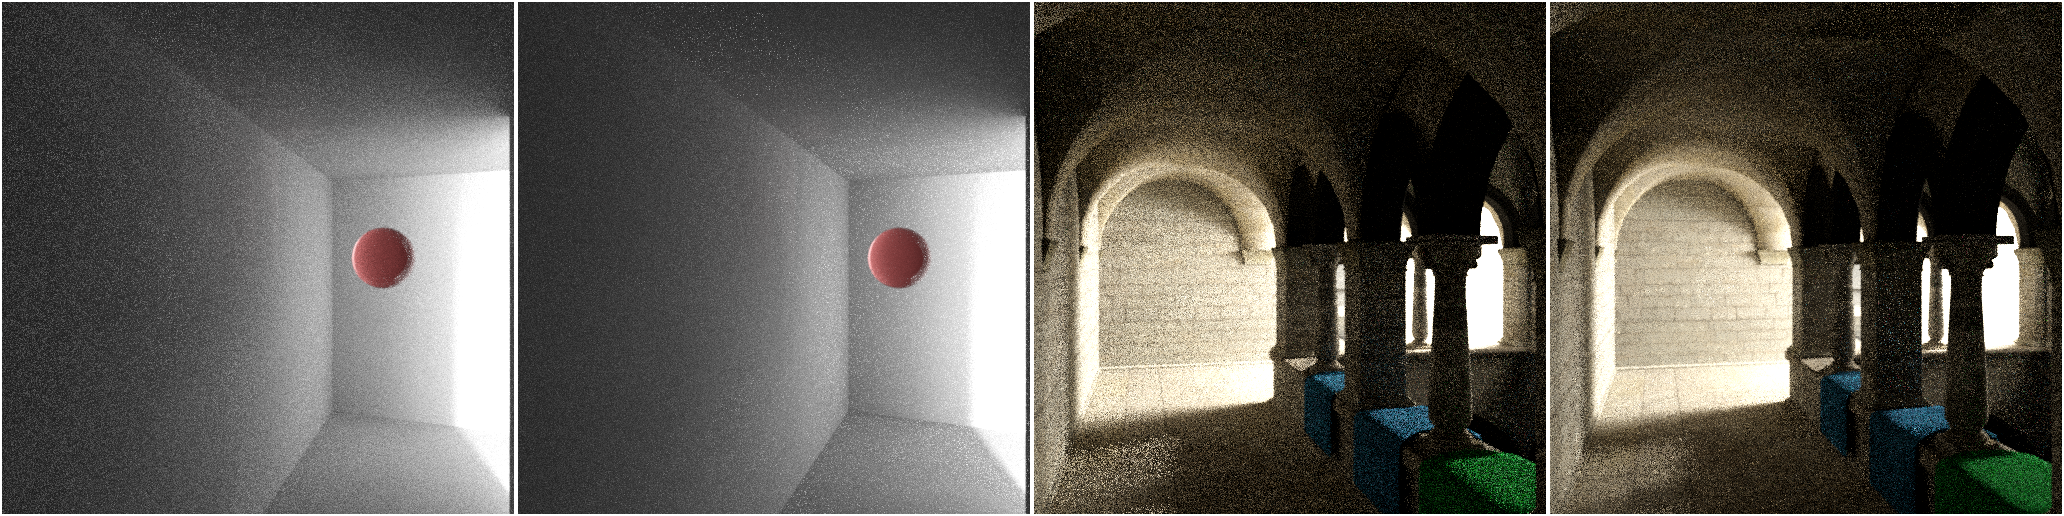
\includegraphics[scale=0.17]{images/four_scenes_for_dgci.png}
\caption{\label{fig:results}Same scene rendered using the classical path tracing (image $a$) or our method (image $b$). Images $c$ and $d$ are both details of respectively images $a$ and $b$ }
\end{center}
\end{figure}

\begin{figure}[tb]
\centering
\begin{tabular}{|c|c|c|c|}
\hline
Scene & Corridor & Sponza 1 & Sponza 2 (Fig. \ref{fig:results}) \\
\hline
MSE 100& 145 / 57 & 301 / 156 & 881 / 826 \\
\hline
MSE 40& 434 / 260 & 924 / 628 & 2678 / 2570 \\
\hline
\end{tabular}
\caption{Time to reach an MSE of 100 and 40 against reference images. In each cell, the left number is for the standard path tracing, the right is for our method}
\label{tab:timing}
\end{figure}

\section{Conclusion}
We presented in this article a new skeletonization algorithm that both preserves geometrical features of objects and produces a pure curvilinear skeleton. These two properties allow us to improve the path tracing algorithm in guiding the rays towards the main illuminated area of the scene. Our algorithm is faster and produce less noise than the classical path tracing method.




\bibliographystyle{splncs03}
\bibliography{./bibli}


\end{document}





